% !TEX root = ../Survey.tex
The Internet is a  large, geographically dispersed network, and information about its structure is needed by all its participants.
Decentralizing the structural information is a key part in its scalability and performance.

Labeling schemes allow the structure of a  graph to be distributed among its nodes  such that certain queries can be answered in a short time.
Moreover, the information needed to answer the queries should be contained in the labels of the questioned nodes themselves.
On the one hand, storing the entire data structure at each node would result in short answer time for each query.
On the other hand, such replications would defy the aim of distributing information.
Therefore, the primary indicator of the quality of a labeling scheme is the size of the labels it produces in the worst-case scenario.

 The papers surveyed are built for specific types of queries. \adjacency \todo{I don't think ``adjacency'' should be written like this all over the place (but it's fine to have it slanted here).} labeling schemes were the first to be investigated in the literature. The nodes in a graph  are labeled in such a way that the \adjacency between two nodes can be determined directly from their labels. A restricted form of \adjacency labeling schemes for graphs was studied almost 50 years ago by \citeN{Breuer67}. The more general concept  was defined 25 years later by Kannan, Naor and Rudich~\shortcite{Kannan92} as well as by \citeN{Muller1988}. Following that, the idea laid dormant for over a decade until it was noticed that labeling schemes could also be defined for many other types of queries other than \adjacency. This observation revived interest in labeling schemes and triggered an abundance of subsequent publications, including many variants of the concept. Further detail on the historical development of labeling schemes can be found in~\cite{Peleg03}.

This survey considers labeling schemes for the family of trees with at most $n$ nodes. We focus on this particular family for the following reasons: 
When graphs are considered, labeling schemes for all of  the  functions we are surveying require a  label size that is in the  order of the size of the graph itself. Even for the most basic query, \adjacency, labeling schemes require at least $n/2$ bits to support the family of  graphs~\cite{rado1964universal}.
It is thus not surprising that the focus of the body of work surveyed, and  the early definitions of labeling schemes,  require labels of a size that is poly-logarithmic in the size of the graph. 
On the other hand, techniques introduced in  the papers surveyed  contributed directly to  labeling schemes for several families of  graphs.
Among others, bounded tree-width~\cite{gavoille2007shorter}, bounded degree~\cite{adjiashvili2014labeling}, bounded arboricity~\cite{Alstrup02}, and planar graphs~\cite{Thorup01} labeling schemes  for various functions are obtained directly from their corresponding labeling schemes for trees. 

\subsection{An example} \label{sec:example}
Before diving into practical applications and details of the precise definition of labeling schemes, it is instructive to warm up with a small example accompanied by some general remarks. 
This section therefore presents a simple \emph{\adjacency labeling scheme for trees}: What this means will be made precise later, but the general idea is to construct an algorithm that associates with every node a \emph{label}, which is just some data, such that, given the labels of two nodes, one can determine if the nodes are adjacent or not.

Consider an arbitrary rooted tree with $n$ nodes. Enumerate the nodes in the tree with the numbers $0$ through $n-1$ as binary strings, and let, for each node $v$, $\Id(v)$ be the number associated with $v$ and, when $v$ is not the root, $p(v)$ be the parent of $v$ in $T$.
Consider the labeling $\la(v)= (\Id(v),\Id(p(v))$ of all non-root nodes $v$ and $\la(\Id(r),\Id(r))$ for the root node $r$.
The encoding of the labels is demonstrated in Figure~\ref{fig:simple}.
Note that two nodes $u$ and $v$ are adjacent if and only if either $\Id(p(v))=\Id(u)$ or $\Id(p(u))=\Id(v)$ but not both. Thus it is possible to determine adjacency of $u$ and $ v$ directly from their labels $\la(u)$ and $\la(v)$.

\begin{figure}[!ht]
\centering
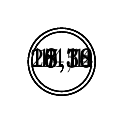
\begin{tikzpicture}[scale = 0.7,inner sep=0pt, minimum size=5ex, sibling distance=0.4em]
\tikzstyle{every node}=[draw,circle]
\Tree  [ 
.{1,1} 
	\edge; [.{2,1} [.{3,2} \edge[]; [.{5,3} \node{6,5}; ]
							       [.\node{7,3}; \node{8,7}; \edge; {9,7} ]
                       					       \edge; [.{10,3} \node{11,10}; ]
					    ] 
					    \edge; {4,2} ]
	\edge;  [.{12,1} \node{13,12}; ]
	[.\node{14,1}; \edge; {15,14}
			[.\node{16,14}; \edge; {17,16}
					[.\node{18,16}; \edge; {19,18}
							\node{20,18};
							\edge; {21,18} ]
					\edge; {22,16} ]
			\edge; {23,14} ]
	]
\end{tikzpicture}
\caption{
A tree with $n=23$ nodes. Each node is assigned a label of size $2 \log n$ supporting \adjacency queries. A node $v$ with parent $u$ is labeled $(\Id(v),\Id(u))$ and the root $r$ is labeled $(\Id(r),\Id(r))$.} \label{fig:simple}
\end{figure}

This is a labeling scheme. It consists of an \emph{encoder} algorithm that labels the nodes of a tree and a \emph{decoder} algorithm that can answer \adjacency queries using only labels as input. Note that the encoding algorithm relies on knowing the entire tree, whereas the decoding algorithm only knows the labels it receives as input and nothing else. 

Recall that the quality of a labeling scheme is measured by the size of the label it produces in the worst case.
In the above example, the pair $(\Id(u),\Id(v))$ can be represented as a binary string of length $2\ceil{\log n}$.\footnote{From hereon, unless stated otherwise,  $\log n$ stands for $ \log_{2} n$}% and $n$ is assumed to be a power of $2$.}
%\todo{Do we really want to assume that $n$ is a power of 2? In principle, you cannot know that such an algorithm works for non-powers of 2 (although it most often will).}
The  goal is to find an \emph{optimal} labeling scheme: that is, one where the worst-case label size is as small as theoretically possible.

There are two main characteristics of a labeling scheme. First, there is the type of query for which the labeling scheme has been constructed. In our example, the type of query is ``\adjacency'', but it could also have been something else, for example ``\ancestry'' (is one node an ancestor of the other?) or ``\distance'' (what is the distance between  two nodes?). Second, there is the family of graphs under consideration. In our example, the labeling scheme is for the family of all trees, but both smaller and larger families would have been possible. A different choice of query or a different choice of graph family may lead to an entirely different labeling scheme with different properties and a different optimal worst-case label size. 

\subsection{Outline}
This survey provides an overview of labeling schemes where the maximum (worst-case) label size is as small as possible.
The problem of finding such labeling schemes for a graph family $\mathcal{G}$  for a given function $f$ is known as the \emph{$f$-labeling problem for $\mathcal{G}$}.
We mainly survey results on  the graph family of trees with at most $n$ nodes due to great interest in the literature, with occasional emphasis on several bounded cases (i.e bounded degree, bounded depth, caterpillars and binary trees).
Tables~\ref{table:main} and~\ref{table:bounded} \todo{Why are tables numerated with Roman numerals? It seems a bit inconsistent.} provide a concise description of the results.
An overview of applications for labeling scheme is provided in Section~\ref{section:applications}, and formal definitions are given in Section~\ref{section:preliminaries}.

Let $k \in \mathbb{N}$, and let $T=(V,E)  \in Trees(n)$ \todo{The ``Trees'' should be a LaTeX command - all over the document...} be a tree rooted at the node $r$.
We survey labeling  schemes supporting  the following functions for any  $u,v,w \in V$:
	\begin{enumerate}
	  \setlength{\itemsep}{2pt}
	\item $\adjacency:(V \times V) \rightarrow \{\false,\true\}$ (Section~\ref{section:Adj})  			 \\ $\adjacency_T(u,v) = \true$ if and only if $u$ and $v$ are adjacent in $T$. \todo{It's totally ugly, in my opinion, that all these functions are slanted. Use $\backslash$operatorname or something.}
	\item $\ancestry: (V \times V) \rightarrow \{\false,\true\}$    (Section~\ref{section:Anc})  		  \\ $\ancestry_T(u,v) = \true$ if and only if $u$ is an ancestor of $v$ in $T$.
	\item $\NCA: (V \times V) \rightarrow \{ 0,1 \}^+$       (Section~\ref{section:NCA})  			\\  $\NCA_T(u,v)$ returns the label of the first node in common for the paths  $v \leadsto r $ and $u \leadsto r$ in $T$.  \todo{Do we need to define and point out the uniquess of ``$\leadsto$''?}
	\item $\routing: (V \times V) \rightarrow \nat $        (Section~\ref{section:Routing})  					\\  $\routing_T(u,v)$ returns the port number (Definition~\ref{dfn:port}) leading to the next node on the  path  $u \leadsto v$ in $T$.
	\end{enumerate}
We also discuss the functions \nonadjacency and \nonancestry which are the negated functions of \adjacency and \ancestry. Each section contains a detailed literature overview,  as well as a report on one or more central results presented in some detail. Common for the algorithms presented is that, in most cases, they are  the best known results.

	Labeling schemes for the following  functions are also reported in Table~\ref{table:main} \todo{I think this table should be properly introduced. Otherwise it's a bit weird to write ``also''.} and occasionally mentioned.
	Some of these functions are also defined for the family of edge weighted $n$ node trees, i.e. trees where each edge is assigned an integer at most $2^M$ for some integer $M$.  We denote this family as $WeightedTrees(n,2^M)$. \todo{``WeightedTrees'' should be a LaTeX command}
	\begin{enumerate}	
	\item $\centerf: (V \times V \times V) \rightarrow \{ 0,1 \}^+$      %(Section~\ref{Section:NCA-lowerbound})
	   \\ $\centerf_T(u,v,w)$  returns the unique node $z$ such that the three paths  $z \leadsto u$, $z \leadsto v$, and  $z \leadsto w$  in $T$ are edge-disjoint.
	\item $\distance: (V \times V) \rightarrow \nat$         %(Section~\ref{section:distance})
	  \\ $\distance_T(u,v)$ returns the length of the path  $u \leadsto v $ in $T$, which is  equal to the number of edges in $u \leadsto v$ if $T$ is unweighted. \todo{Do we need to define ``length of the path'' in the weighted case?}
	\item $\flow: (V \times V) \rightarrow \nat$         %(Section~\ref{section:distance})   	
	\\ $\flow_T(u,v) $ returns the smallest edge weight on $ u \leadsto v$  in $T$.
	\item $\siblings: (V \times V) \rightarrow \{false,true\}$       % (Section~\ref{section:Sib}) 
	 \\ $\siblings_T(u,v) = true$ if and only if  the parent of $u$ is the parent of $v$ in $T$ for $u \neq r$ and $v \neq r$. A node is its own sibling. \todo{I'm not sure that is the standard definition. The labeling problem is different in the two cases---uniqueness is not required!}
	\item $\seplevel: (V \times V) \rightarrow  \{ 0,1 \}^+$        (Section~\ref{sec-NCA-FIXED}) 			  \\ $\seplevel_T(u,v)$ returns the length of the path  $r \leadsto w $ in $T$ where $r$ is the root and $w$ is $NCA_T(u,v)$.
	\item $\smalldistance: (V \times V \times \nat) \rightarrow \nat$    
	\\ $\smalldistance_T(u,v,k)= true$  if and only if $\distance_T (u, v) \leq k$ in $T$, otherwise, it returns $\infty$.
	\end{enumerate}
	
See Figure~\ref{fig:complexityruler} for an illustration of the number of bits required for labeling schemes for each of these functions.
In the course of the survey, we provide missing details and correct minor mistakes found in the literature surveyed.
We also present an improved labeling scheme for the function \ancestry in Section~\ref{subsetion:mat-optimal}.

\begin{table}
\tbl{Known upper and lower bounds for efficient  labeling schemes on trees. Labeling schemes that do not necessarily provide unique labels  are marked with *.The families  $Trees(n), Forests(n), BinaryTrees(n),Trees(n, \delta)$ and $Trees(n, \Delta)$ are formally defined in Section~\ref{section:preliminaries}. Results implied, but not specified in the literature are marked with $^{\dagger}$.}{
\begin{tabular}{cccccc}
    Reference &Variant  & Upper bound	&Lower bound	  & Encoder & Decoder    \\ \hline\hline
&&\underline{\adjacency} \\ \\
\cite{alstrup2015optimal}		&$Trees(n)$  &$\log n+O(1)$ 		&$\log n+ 1$ 			 &$O(n)$ 			& $O(1)$\\ 
\cite{Gavoille06} &$BinaryTrees(n)$    &$\log n+O(1)$  		 &$\log n+ 1$		 	& $O(n)$	            	&$O(1)$ \\ 
\cite{Fraigniaud10}	&$Trees(n, \delta)$ 		  &$\log n+3 \log \delta+O(1)$   &$\log n+ 1$	& $O(n)$	            	&$O(1)$  \\ 	
\cite{adjiashvili2014labeling}	&$Trees(n, \Delta)$ 	   &$\log n+O(\log \Delta)$  &$\log n+ 1$	& $O(n \log n)$	            	&$O(\log\log n)$\\ 						
			
%			 &One sided error*			& $2(k+1) $ with	 	  					& $\log n + \log p - O(1)$	 & $O(n)$ 		        & $O(1)$ 			&\cite{fraigniaud2009} \\ 
%			&   						&$p= 1-\frac{1}{2^k}$						&		\\ 
&&\underline{\nonadjacency} \\ \\
\cite{fraigniaud2009} &One sided error* & $2k+1$ with 	&$---$	 & $O(n)$ 		        & $O(1)$ \\ 
&&$p= 1-\frac{1}{2^k}$\\ 	\hline
&&\underline{\ancestry} \\ \\
\cite{dahlgaard2014improved}&$Trees(n)$	 &$\log n +2 \log \log n+3$	 	  		&$\log n+ \log \log n$& $O(n)$ 		        & $O(1)$ \\ 
\cite{Fraigniaud10} &$Trees(n,\delta)$	&$\log n +2 \log \delta+ O(1) $	&   & $O(n)$ 		        & $O(1)$ \\ 
\cite{fraigniaud2009}	&One sided error*   			& $\log n - \frac{k}{2}+ O(\log \log n)$& $\log n + \log p -$	& $O(n)$ 	& $O(1)$ \\ 
&& with $p=\frac{1}{2^k}$	&$O(1)$\\ 				
&&\underline{\nonancestry}\\ \\
\cite{fraigniaud2009}&One sided error*  & $\lceil \log n \rceil $ with 	& $\log n + \log p -$	 & $O(n)$ 		        & $O(1)$ \\ 
&&  $p=\frac{1}{2}$	&$O(1)$\\ \hline			
&&\underline{\centerf} \\ \\
\cite{Peleg05} &$Trees(n)$, fixed model &$\Theta(\log^2 n)$ 	&$ \Theta(\log^2 n)$		 & $O(n \log n )$	  		&$O(1)^{\dagger}$ \\ \hline
&&\underline{\connectivity}\\ \\ 
 \cite{Alstrup05} &$Forests(n)$		&$\log n+\log\log n  $ & $\log n+\log\log n$ 	 & $O(n)$	  		&$O(1)$ \\ 
 \cite{Alstrup05} &$Forests(n)  $*	&$\log n $		 		& $\log n$ 	 & $O(n)$	  		&$O(1)$ \\ \hline

&&\underline{\distance}\\ \\	
\cite{freedman2016optimal}&$Trees(n)$   &$\frac{1}{4}\log^2 n+o(\log^2 n)$  &$\frac{1}{4}\log^2 n - O(\log n)$  & $O(n \log n)$     & $O(1)^{\dagger}$\\ 
\cite{Gavoille2001}&$WeightedTrees(n,2^M)$  &$\Theta(M \log n + \log^2 n)$	&$\Theta(M \log n + \log^2 n)$	  & $O(n \log n)$    & $O(\log n)$\\  \hline

&& \underline{\distance, approx. $1+1 / n$} \\ \\
\cite{Katz00} &$2^M$ weighted diameter &$\Theta(\log n \cdot \log M)$ 	&$\Theta(\log n \cdot \log M)$ 	 & $O(nm)$ & $O(1)$ \\ 
\cite{Katz00}& $Trees(n)$	&$\Theta(\log n \cdot \log \log n )$&$\Theta(\log n  \log \log n)$  &$O(n \log n)$ &$O(1)$\\ 	\hline
		
&&\underline{\flow} \\\\
\cite{katz2004labeling}&$WeightedTrees(n,2^M)$  &$\Theta(M \log n + \log^2 n)$  &$\Theta(M \log n + \log^2 n)$	& $O(n)$    & $O(1)$ \\ \hline

&&\underline{\NCA} \\ \\
\cite{Green14}&$Trees(n)$, \NCAl	&$ 3 \log n$	&$1.008\log n $	& $O(n)$	     		& $O(1)$ \\ 
\cite{Peleg05}&$Trees(n)$, \NCAf			 &$O(\log^2 n)$	  &$\Omega(\log^2 n)$ 		 & $O(n \log n)$	& $O(1)^{\dagger}$ \\ \hline

&&\underline{\routing} \\ \\
\cite{Thorup01}&$Trees(n)$, designer port  &$(1+o(1))\log n$  & $\log n + \log \log n$ 		& $O(n \log n)$	  		&$O(1)$  \\ 
\cite{Fraigniaud01}&$Trees(n)$, fixed port	  & $\Theta(\log^2 n/\log\log n) $  & $\Theta(\log^2 n/\log\log n)$ 	 & $O(n)$	  &$O(1)$  \\ \hline

&&\underline{\siblings} \\ \\ 
\cite{lewenstein2013succinct}&$Trees(n)$	&$\log n+ \log\log n $	& $\log n+ \log\log n$ 	 & $O(n)$	  		&$O(1)$ \\ 
\cite{Alstrup05}	&$Trees(n)$*	&$\log n $		 & $\log n$ 	 			& $O(n)$	  		&$O(1)$  \\ \hline
						
&&\underline{\smalldistance} \\ \\
\cite{freedman2016optimal} &$Trees(n)$,distance $k$  &$ \min{\log n+O(k \log (\log n/k))} $	&$\log n+\Omega(k \log(\log n/(k \log k)))$	  & $?$    & $O(1)$\\ 
&&	$O(\log n \cdot \log(k/\log n))$	 \\  \\		 
  \end{tabular}} \label{table:main}
\end{table}

				\begin{figure}
				\centering
				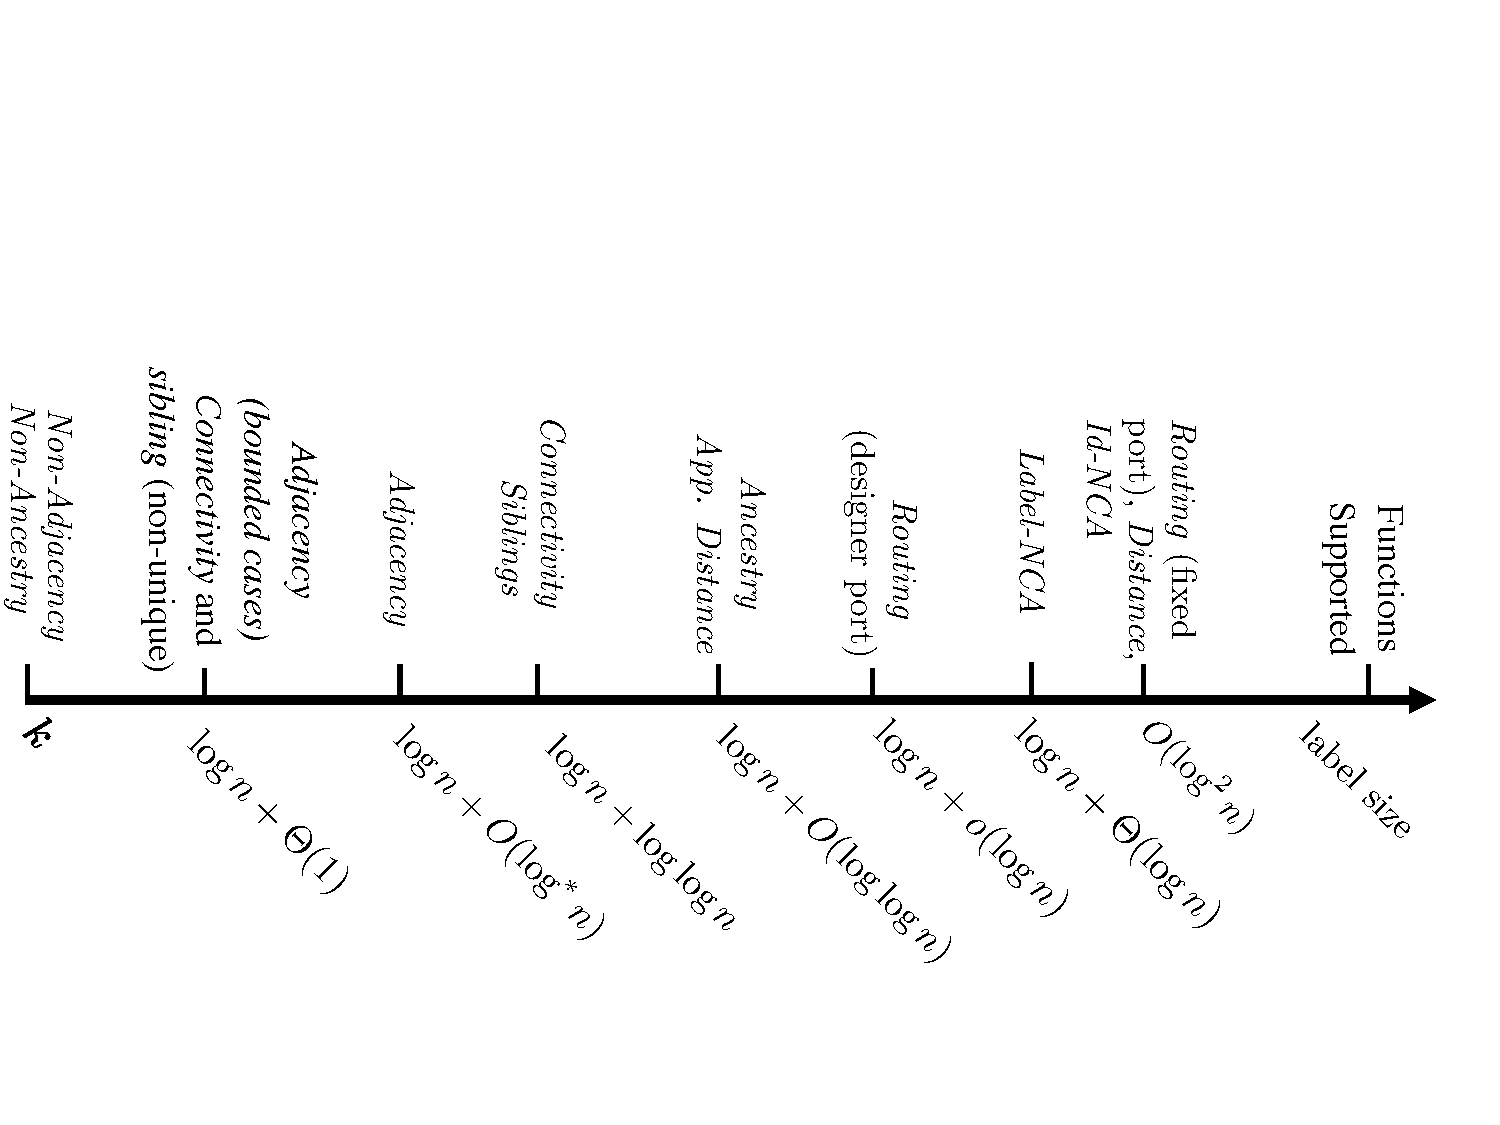
\includegraphics[width=100mm]{./Figures/Hierarchy2.pdf}
				\caption{Given a certain label size, the illustration describes  which operations may be  supported.  }
				\label{fig:complexityruler}
			\end{figure}
			
\todo{Comment to Table I: There is also a less efficient NCA labeling scheme with smaller labels}

\paragraph{Bounded trees}\label{section:Limited}
In Table~\ref{table:bounded}  we complete the description of the following cases: $Caterpillars(n)$, $Trees(n,\delta)$, $Trees(n,\Delta)$, and  $BinaryTrees(n)$, where $\Delta$ refers to maximum degree, $M$  to $2^M$ edge weights, and $\delta$  to  maximum depth.
Note that the table is transposed compared to Table~\ref{table:main}.
We chose to present the results in this fashion  since the  focus is  on the restricted families.
\begin{table}[!ht]
\tbl{Known upper and lower bounds for  labeling schemes on trees with unique encoder.}{
  \begin{tabular}{lcccccc}
    \hline
    &\adjacency 			  & \ancestry		 &\distance			 & \NCA	  		& \siblings   \\ \hline
    \hline
$Caterpillars(n)$: \\
Upper bound	&$\log n +\Theta(1)$  &$\log n +O(1)$  &$2 (\log n + M) $	&$\log n + \log \log \Delta + O(1) $ 	 	&$\log n +O(\log \log n)$\\
& \cite{Gavoille06}	 &  & && \cite{Alstrup05}  \\	\hdashline	

Lower bound	&$\log n + \Theta(1)$ &	$\log n + \Theta(1)$		 &$\log n + \Theta(1)$&	$\log n + \Theta(1)$	& $\log n +\Omega(\log \log n)$	\\ 
&&&&&\\ \hline 

$BinaryTrees(n)$:\\
Upper bound &$\log n +O(1)$ 	 &$\log n +\Theta(\log \log n )$  &$\frac{1}{2}\log^2 n +O(\log n)$&$ O(\log n)$\cite{Alstrup02NCA}&$ \log n +\Theta(1)$  \\ 
&\cite{Gavoille06}	&[Fraigniaud et al. 2010b]&\cite{Gavoille2001}	&\cite{Alstrup02NCA}	&\\ \hdashline   
Lower bound		&$\log n + \Theta(1)$					&$\log n +\Theta(\log \log n)$	  	    &$\frac{1}{8}\log^2 n-O(\log n)$&$\log n + \Theta(1)$	&$\log n + \Theta(1)$	\\ 
&&	&\cite{Gavoille2001}	&		&	\\ \hline 
				
$Trees(n,\Delta)$:\\
Upper bound 	&$\log n +O(1)$ & $\log n +\Theta(\log \log n) $ & $\frac{1}{2}\log^2 n +O(\log n)$ & $O(\log n)$ &$\log n + \Theta(\log \log \Delta)$\\ 
&[Adjiashvili et al. 2014]& [Fraigniaud et al. 2010b] &\cite{Gavoille2001}&\cite{Alstrup02NCA}&\cite{Alstrup05} \\\hdashline

Lower bound &$\log n + \Theta(1)$ &$\log n + \Theta(1)$ &$\frac{1}{8}\log^2 n-O(\log n)$  &$ \Omega(\log n)$	&$\log n$	\\ 
&&&\cite{Gavoille2001}&\cite{Alstrup02NCA} \\
\hline 
			
$Trees(n,\delta)$:\\
Upper bound & $\log n + 3 \log d +O(1)$ &$\log n +2 \log \log d +O(1) $ &$\frac{1}{2}\log^2 n +O(\log n)$ 	&$\log n +O(1)$ 	&$\log n+ \Theta(\log \log n)$\\ 
& [Fraigniaud et al. 2010b] &[Fraigniaud et al. 2010b]	&&& \cite{Alstrup05}\\	\hdashline				

Lower  bound & $\log n + \Theta(1)$	&$\log n + \Theta(1)$  &$\log n + \Theta(1)$  &$\log n + \Theta(1)$  &$\log n + \Theta(\log \log n) $  \\ 
&&&&& \\ \hline						
  \end{tabular}}\label{table:bounded}
\end{table}

\todo{Comment to Table II: It's not the encoder that is ``unique''}	

\todo{Comment to non-existing table: What about all the other variations of labeling schemes, e.g. approximation, probabilistic etc.?}	

						
\subsection{Practical and theoretical applications of labeling schemes}\label{section:applications}
Labeling schemes have  contributed directly to a number of areas, including XML querying, graph theory, shortest paths in road networks and routing schemes.

\paragraph{XML querying}  
 Extensible Markup Language (XML) documents are a popular and ubiquitous standard for exchanging structured data on the Internet~\cite{Kaplan01}. An XML document can be viewed as a rooted tree in which each node corresponds to a semantic element, enclosed by matching beginning and end tags in the form $\verb+<item>+\dots\verb+</item>+$. When searching for information in an XML document, one will typically not only search for pure text but also utilize the semantic structure of the document and specify, for example, certain ancestry relations in the document tree. By using a labeling scheme, queries of this type can be answered directly from labels, which can be stored in a hash table, without having to access the actual document. 
 This can have a significant positive impact on performance, and has been studied extensively~\cite{Cohen02,lu2013xml,harder2007node,Kaplan01,wu2004prime,cohen10journal}.

To achieve a good performance for  queries on  XML documents, it is important  that a large  part of the document's indexed structure can reside in main memory. Since these structures can be extremely large, every single bit counts.
Much of the work in this particular direction focused on seemingly small benefits. For example, both relations used by practitioners, namely, adjacency (illustrated in Figure~\ref{fig:simple}) and ancestry  had strikingly simple  labeling schemes with labels of at most $2 \log n$ bits~\cite{Kannan92}.
In order to identify the XML element uniquely, the label of an element  in an XML file with at most $n$ elements requires at  least  $\log n$ bits. 
The effort to reduce the single additive $\log n$ \todo{You just argued that it cannot be reduced. I guess you mean everything in addition to the $\log n$.} contributed  not only to the performance of XML queries but also to the subject of implicit representation of trees.

\paragraph{Graph theory}
If the query type supported by a labeling scheme allows the entire graph to be reconstructed from the labels, then the collection of labels can be seen as an \emph{implicit representation} of the graph: that is, a representation where the graph is not stored as a single structure but can be determined from a collection of smaller structures.
This is in contrast to any global representation of a graph, for example an adjacency matrix, where the adjacency between two nodes is determined by consulting the relevant entry in a single entity, and where the index of each node contains no relevant information in itself but serves only as a placeholder or a pointer to the entries of the matrix. 
In this sense, a labeling scheme is more efficient since it does not waste space on meaningless placeholders. This, however, does not mean that the collection of labels in total uses less space than a traditional representation: on the contrary, the extra requirement that the data structure must be distributed may lead to one that is  larger in total. 

\citeN{Kannan92} noticed the tight correlation between adjacency labeling schemes and induced-universal graphs. Induced-universal graphs is  a mathematical subfield of implicit graph representations and has been researched extensively since the 1960's~\cite{rado1964universal}. 
For various numbers of families, the goal is to find the smallest number of nodes required for a graph that contains each of the $n$-node graphs of the family  as induced subgraphs. 
 A subsequent connection between universal matrices and \distance labeling schemes was studied by \citeN{Rodeh10} and \citeN{Paul01}.
We defer further discussion on the nature of the connection to Section~\ref{section:Adj}.

\paragraph{Shortest paths in road networks}
Another practical aspect of labeling schemes concerns distributed shortest paths  on road networks. 
\citeN{Gavoille2001} first investigated \distance labeling schemes. 
Abraham, Deiling, Goldberg and Werneck \shortcite{abraham2010hub,abraham2012hierarchical} modified the labeling schemes to achieve a distributed system to answer reachability and shortest path queries on road networks.

\paragraph{Routing schemes}
Perhaps the most  practical application of labeling schemes arises from  routing schemes.
In a large network, information sent from one participant  to another must visit   other participants in the network according to the network topology. 
A routing scheme is a description of a  system designed to support the operation of transferring packets through the network.
According to \citeN{Peleg05}, labeling schemes  assist in the design of ``memory-free'' routing schemes, which support fast and simple switch architectures by  storing  little data locally.
 A significant effort by the community yielded numerous  papers dealing with labeling schemes for routing \cite{Peleg03,Thorup01,Fraigniaud01,gavoille96,Dom07,Korman07K,krioukov2004compact,abraham2006routing,abraham2005name}.





\subsection{Preliminaries}\label{section:preliminaries}
In the remainder of the paper we use the following terms:
			$k$ is a positive integer.
			A binary string is a member of the set $\{ 0,1 \}^*$.
			We define $\ceil { \log_2{n}}$ as $\log{n}$.   %\todo{Really? Maybe you mean that we \emph{define} $\log n$ to mean $\ceil{\log_2 n}$?}
			We denote by $\mathbb{N} = \{1,2 \dots \} $ the set of natural numbers and by $\mathbb{N}_0 = \{0,1,2 \dots \} $ the extended set that includes $0$.
			For $x \in \mathbb{N}$ we denote by $\bin(x)$ its standard binary representation, and $\vert x \vert$ as the number of bits in $\bin(x)$. \todo{The latter seems like a really dangerous and weird definition. Then we have e.g. $\vert 4\vert=3$.}
			The concatenation of two bit strings $a$ and $b$ is denoted $a \circ b$.
			\subsubsection{Graph families related definitions} 
			For a graph $G$ we denote the set of nodes and edges by $V(G)$ and $E(G)$, respectively.
			For any graph family $\mathcal{F}$, let $\mathcal{F}(n) \subseteq \mathcal{F}$ denote the subfamily containing the graphs of at most $n$ nodes.
			Unless stated otherwise, the number of nodes in a graph $n$ is assumed to be a power of $2$. \todo{Again, I think this is somewhat restrictive}
			The family of all graphs is denoted $\mathcal{G}$.
			 The collection of unweighted forests in $\mathcal{G}$ respectively~$\mathcal{G}(n)$  is  denoted $Forests$ respectively~$Forests(n)$. \todo{Make a LaTeX command for ``Forests''}
			The collection of unweighted trees in $Forests$ respectively~$Forests(n)$  is  denoted $Trees$ respectively~$Trees(n)$.
			Similarly,  the  collection of edge weighted trees, with weights in $\{1 \dots 2^M \}$  in $\mathcal{G}$ respectively~$\mathcal{G}(n)$ is denoted $WeightedTrees(2^M)$ respectively~$WeightedTrees(n,2^M)$.
			A \emph{caterpillar} is a tree in which all non-leaf nodes lie on a single path, denoted the \emph{main path}. The collection of unweighted caterpillars in $Trees$ respectively~$Trees(n)$  is denoted $Caterpillars$ and $Caterpillars(n)$.
			The collection of trees with bounded depth $\delta$ in $Trees$ respectively~$Trees(n)$  is  denoted $Trees(\delta)$ respectively~$Trees(n,\delta)$.
			Trees of  Bounded degree $\Delta$  are marked similarly $Trees(\Delta)$  and $Trees(n,\Delta)$.
			As a shorthand, trees of bounded degree $3$ are marked $BinaryTrees$ and $BinaryTrees(n)$. \todo{If trees are rooted, this may not be the correct definition}
			For each of the (unbounded) families described the bounded degree and depth variants are denoted in according.
			From hereon, unless stated otherwise, we assume trees to be rooted. 

	\subsubsection{Basic tree related definitions} \label{definitions-of-trees}
	Let $T=(V,E) \in Trees(n)$ be a tree rooted in $r$. The number of edges in a tree is always $|E|=|V|-1$. The nodes of degree $1$ other than the root are called \emph{leaves}, and all other nodes are called \emph{internal} nodes.
	
	Let $u$ and $v$ be nodes in  tree $T$. 
	If $(v,u) \in E$ \todo{Since edges have no direction, I think the correct definition would be $\{v,u\}$} we say that $v$ and $u$ are  \emph{neighbours}. We denote  the set of all neighbours of $v$ as $N(v)$, and the degree $\vert N(v) \vert$ of $v$ as $\deg(v)$.  A non-root node with degree at most $1$ is called a  \emph{leaf}, and an \emph{inner node} is a non-leaf node. The parent of $v$, if $v$ is not the root, is denoted $p(v)$, and $v$ is the \emph{child} of $p(v)$.  A \emph{sibling} $v \neq u$ of $u$  is a child of $p(u)$.
	We denote by $v \leadsto u$ the  sequence  \tuple{v_0,v_1 \dots v_k} of vertices such that $v = v_0$, $u = v_k$, and $(v_{i-1},v_{i})\in E$ for $ i= 1,2 \dots k$ between $v$ and $u$ in $T$. \todo{Can there be duplicates? If yes, then paths are not unique.}
	This sequence is typically called the \emph{path} between $v$ and $u$, and $k$ is called the \emph{length} of the path $v \leadsto u$. Note that   every two nodes in a tree are connected by a unique path.
The distance between $u$ and $v$ in $T$, denoted $\distance(u, v)$, is the number of edges on the path  $u \leadsto v $. The distance from  $v$ to the root is called the \emph{depth} of $v$, denoted $\depth(v)$, and the depth of the tree, $\depth(T)$, is the maximum depth among its nodes.
	If $u$ is a node on the path from the root of a rooted tree to a node $v$, then $u$ is an \emph{ancestor} of $v$, and $v$ is a \emph{descendant} of $u$. Note, in particular, that a node is its own ancestor, descendant and sibling, but not its own child or parent. A \emph{common ancestor} of two nodes is a node that is an ancestor of both nodes, and their \emph{nearest common ancestor} (NCA) is the unique common ancestor with maximum depth. Given a node $v$, the descendants of $v$ form an induced subtree $T_v$ with $v$ as root.  Finally, the \emph{size} of $v$, denoted $\size(v)$, is the number of nodes in $T_v$.
	
	Additional standard definitions are provided in Appendix~\ref{AppendixA}.
\subsubsection{Labeling schemes and variations} 
We present definitions of labeling schemes, approximation labeling schemes and one-sided error labeling schemes.			
\begin{definition}\label{dfn:labeling_schemes}
Let $f : V(G)^k  \rightarrow S$ be a k-ary function  over nodes in  $G \in \mathcal{G}$ into $S$.


A \emph{label assignment} $e_G$  for $G \in \mathcal{G}$ is a mapping of each $v \in V(G)$ into a bit  string $e_G(v)= \la(v)$, called  the \emph{label} of $v$. \todo{Why do you need two notations for the same thing?}

An  \emph{f-labeling scheme} for  $\mathcal{G}$, denoted  $\tuple{e,d}$, \todo{Why these strange brackets?} consists   of the  following:
	\begin{enumerate}
		\item An \emph{encoder} $e$ which is an algorithm that  receives  $G \in \mathcal{G}$ as input and  computes the label assignment $e_G$. 
		 \item A \emph{decoder}  $d$ which is an algorithm  that  gets  any sequence of $k$ labels  $\la(v_1)\dots \la(v_k)$  and computes the query $d(\la(v_1)\dots \la(v_k))$.
		 If  $d(\la(v_1)\dots \la(v_k))=f(v_1\dots v_k)$ we say that $d$ is an \emph{exact} decoder.
	\end{enumerate}
\end{definition}

\begin{remark}  \label{remark:unique}\mbox{}
		\begin{enumerate}[i.]
			\item If, for all $G \in \mathcal{G}$, $e_G$ is an injective mapping, i.e. for all distinct $u,v \in V(G)$, $e_G(u) \neq e_G(v) $, we say that the labeling scheme has a \emph{unique} encoder.
			\item The encoding of a node depends on the graph to which the node belongs, whereas the decoding of a k-tuple of labels is oblivious to the graph from which the labels come.
			\item By Definition~\ref{dfn:labeling_schemes} labels of unrestricted size can be used to encode the entire graph structure.
		
		\end{enumerate}
\end{remark}



\begin{definition}
	Let  $\tuple{e,d}$ be an $f$-labeling scheme  for  $\mathcal{G}(n)$.
	\begin{enumerate}
		\item   $\tuple{e,d}$  is a \emph{$\rho(n) \, f$-labeling scheme} if  for  any $G \in \mathcal{G}(n)$,  the size  of any label in the  label assignment $e_G$  is bounded by some function $\rho(n)$. 
		\item $e$  is  \emph{computed in time $t(n)$} if for any $G \in \mathcal{G}(n)$, $e$ computes the label assignment $e_G$  in time at most $t(n)$. \todo{Do we actually measure time for the whole graph and not just individual nodes?}
		\item  $d$ is  \emph{computed  in time $t(n)$}  if for any $G \in \mathcal{G}(n)$  and any $v_1\dots v_k \in G$  the query $d(\la(v_1)\dots \la(v_k))$ is computed in time at most $t(n)$.
				\item   $\tuple{e,d}$  is an \emph{average $\rho \, f$-labeling scheme}  if for  any  $G \in \mathcal{G}(n)$,  the sum of lengths of all labels in the  label assignment $e_G$  is bounded by $\rho(n) \cdot n$ (See \cite{Kano07}). 
	\end{enumerate}

\end{definition}


We turn to define labeling schemes that provide an approximate solution.
\begin{definition} \label{dfn:approx-label}
Let $f : V(G)^k  \rightarrow \nat$ be a k-ary function  over nodes in  $G \in \mathcal{G}$ to $\nat$.
An \emph{R-approximate}  $f$-labeling scheme for $\mathcal{G}$, denoted  $\tuple{e,d}$, is an $f$-\emph{labeling scheme} with the following property.
Consider any graph $G=(V,E) \in \mathcal{G}$ which receives a label assignment $e_G$ from $e$. Then for any set of nodes $v_1\dots v_k\in V$ with labels  $\la(v_1)\dots \la(v_k) $ the value computed by $d$ satisfies 
\todo{Is this the standard definition? I would have thought that the lower bound did not divide by $R$. Also, what about additive errors, which we will need for distances?}
\[ \frac{1}{R} \cdot d(\la(v_1)\dots \la(v_k)) \leq  f(v_1\dots v_k) \leq {R} \cdot d(\la(v_1)\dots \la(v_k)).   \]
\end{definition} 

We also define the forbidden-set variant \cite{courcelle2007forbidden}.
\begin{definition}\label{dfn:forbidden}
				Let  $f$ be a boolean function over node sets  in  $G \in \mathcal{G}$ to $\nat$, and let $X$ be a subgraph of $G$.
				 A \emph{forbidden-set $f$-labeling scheme } is an $f$-labeling scheme (Definition~\ref{dfn:labeling_schemes})  where the decoder receives the subgraph $X$ and returns $d(\la(v_1) \dots \la(v_k))$ where the function is defined over the graph $G \setminus X$.
\todo{I simply don't understand this definition. What is this used for? And did we even define ``subgraph'' anywhere (should it be node-induced etc.?}		
			\end{definition}


Finally we define the one-sided error variant  \cite{fraigniaud2009}.

			\begin{definition}\label{dfn:one-sided}
				Let  $f$ be a boolean function over node sets  in  $G \in \mathcal{G}$ to $\nat$.
				 A (probabilistic) \emph{one-sided error $f$-labeling scheme  with guarantee $p$} is an $f$-labeling scheme (Definition~\ref{dfn:labeling_schemes})  with the following property:
				 Consider any graph $G=(V,E) \in \mathcal{G}$ which receives a label assignment $e_G$ from $e$. Then for any set of nodes $v_1\dots v_k\in V$ with labels  $\la(v_1)\dots \la(v_k) $
				 \begin{itemize}
				 	\item  If  $f(v_1\dots v_k) = \true $,  then   $prob(d(\la(v_1)\dots \la(v_k)) = \true) \geq p$. 
				 	\item If  $f(v_1\dots v_k) = \false$, then $d(\la(v_1)\dots \la(v_k)) = \false$.    
				 \end{itemize}
			\end{definition}
			
	From hereon, unless stated otherwise, encoder and decoder stand for exact decoder and deterministic encoder. \todo{I don't think we have defined non-deterministic encoders anywhere?}
		
		Denote the family of trees with at most $n$ nodes $total(n)$ and the family of trees with exactly  $n$ nodes $exact(n)$.
		In the literature reviewed, some  results \cite{Kaplan01,Kannan92} are defined  for $total(n)$,  while other \cite{Alstrup02,Korman07K,gavoille07,Alstrup05} are defined  for $exact(n)$.
		Naturally, for $n>1$, $exact(n) \subset total(n)$.
		Therefore, upper bounds defined for $total(n)$ trivially hold for $exact(n)$.
		In contrast,  lower bounds on labeling schemes for $exact(n)$ hold for $total(n)$.
		It may be conjectured that for labeling schemes, the  definitions are equivalent, but  there exist no such proof in the literature surveyed.
		The subject is expended in \cite{Esben13}. 
		We were unable to find a labeling scheme or a lower bound for a labeling scheme in which the result provided only holds for either $exact(n)$  or $total(n)$. \todo{HUH? I can trivially do that!}


%\footnotetext{See Definition~\ref{dfn:tree-things-app}. In addition, for $Trees(n)$, M=$\log n$} 

 	
